\section{Module 1: Bảng điều khiển Horizon \& Vòng đời Dịch vụ Cốt lõi}

\subsection{Mục tiêu \& Khảo sát Ban đầu}
Trong Module 1, nhóm chúng em tiến hành kiểm tra và xác nhận trạng thái hoạt động ban đầu của toàn bộ nền tảng OpenStack ngay sau khi hoàn tất quá trình cài đặt bằng DevStack. Mục tiêu của bước này là thiết lập đường cơ sở (Baseline) tin cậy cho các lớp dịch vụ điện toán, lưu trữ và mạng, đồng thời làm quen với các thao tác quản trị trên cả giao diện đồ họa Horizon lẫn công cụ dòng lệnh OpenStack CLI.

\subsection{Kiểm tra Hiện trạng Dịch vụ Cốt lõi}
Đăng nhập vào bảng điều khiển Horizon dưới ngữ cảnh dự án \texttt{demo}, nhóm chúng em đã tiến hành khảo sát toàn diện hiện trạng của các dịch vụ:

\begin{figure}[H]
\centering
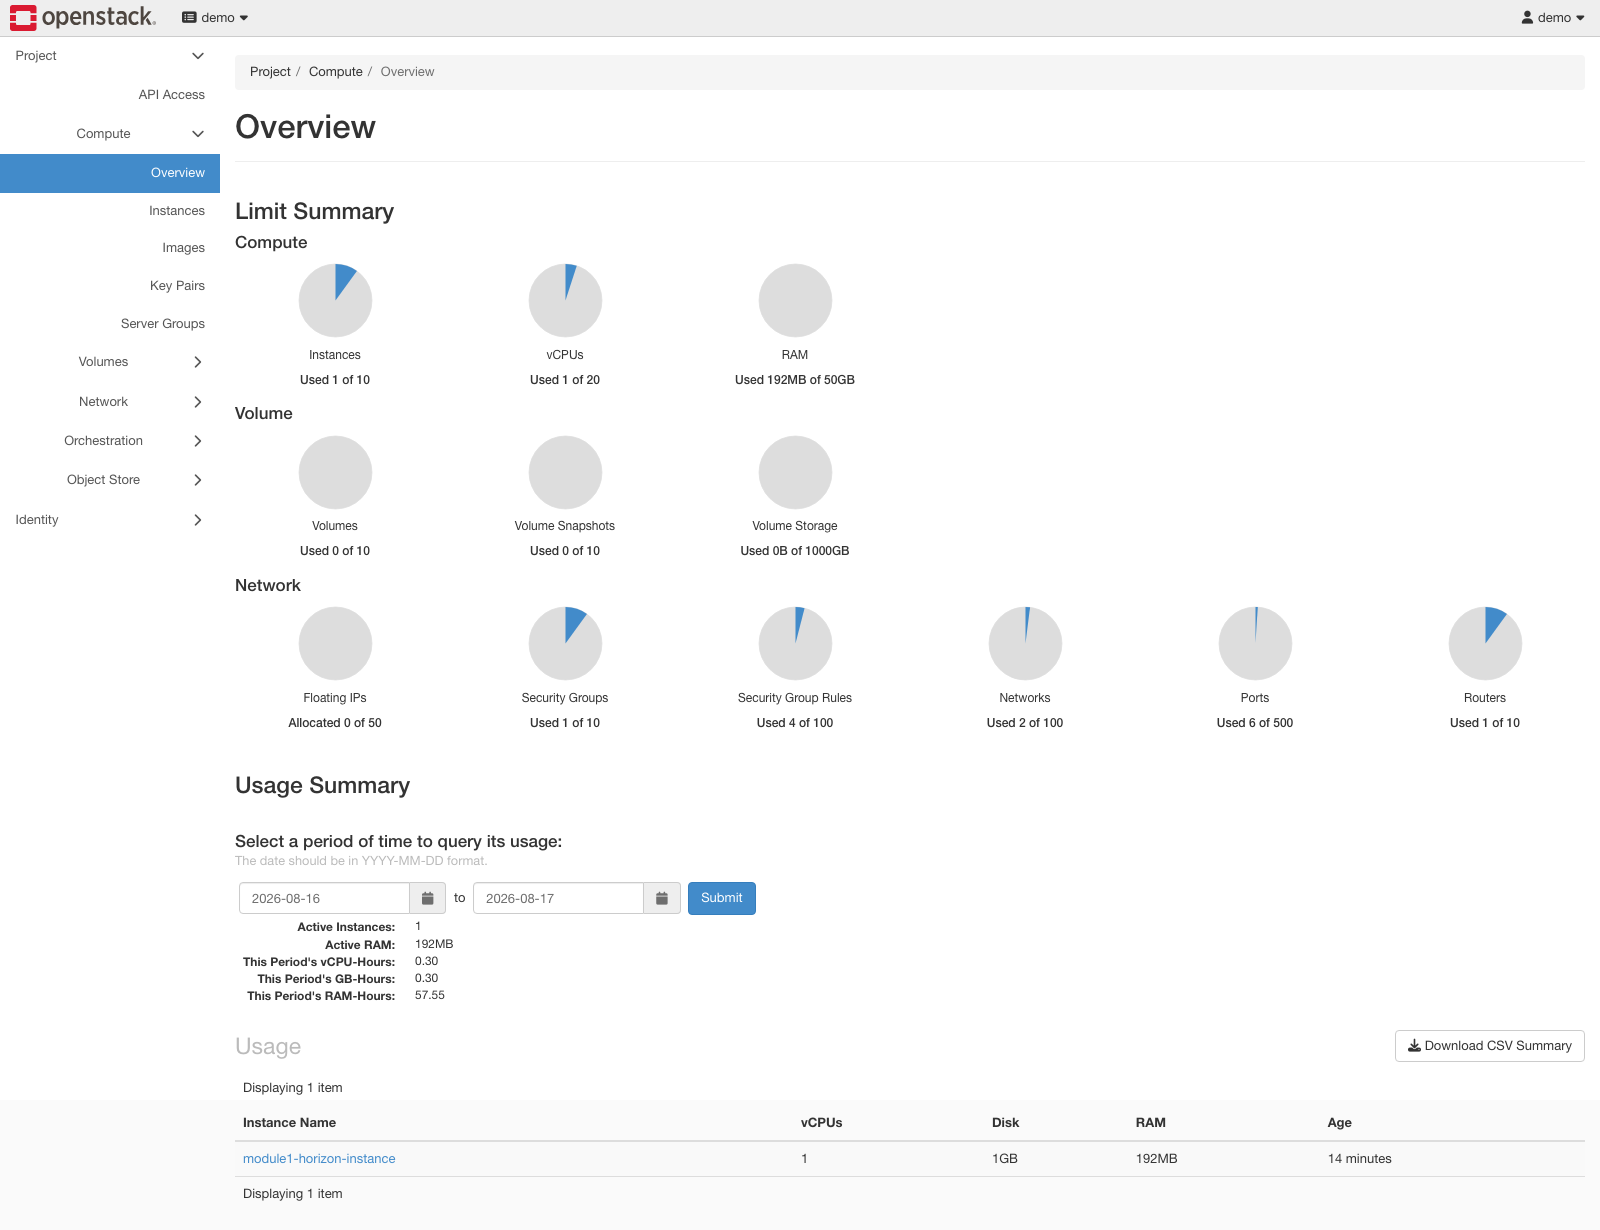
\includegraphics[width=0.88\linewidth]{img/m1-compute-resource-overview.png}
\caption{Giao diện Compute Overview và tổng quan hạn ngạch tài nguyên dự án.}
\label{fig:m1_overview}
\end{figure}

\begin{itemize}
    \item \textbf{Tổng quan Điện toán (Hình~\ref{fig:m1_overview}):} Nhóm ghi nhận hạn ngạch (Quota) mặc định của dự án gồm 10 Instances, 20 vCPUs, 50 GiB RAM, 1000 GiB Volume Storage và 50 Floating IPs.
    \item \textbf{Danh mục Ảnh máy ảo (Hình~\ref{fig:m1_glance_images}):} Dịch vụ Glance đã tích hợp sẵn hai ảnh máy ảo phục vụ thử nghiệm: bản CirrOS siêu nhẹ \nolinkurl{cirros-0.6.3-x86_64-disk} (20.69 MB) để kiểm thử nhanh và bản \nolinkurl{Fedora-Cloud-Base-37-1.7} (470 MB) cho các tác vụ Linux đầy đủ.
\end{itemize}

\begin{figure}[H]
\centering
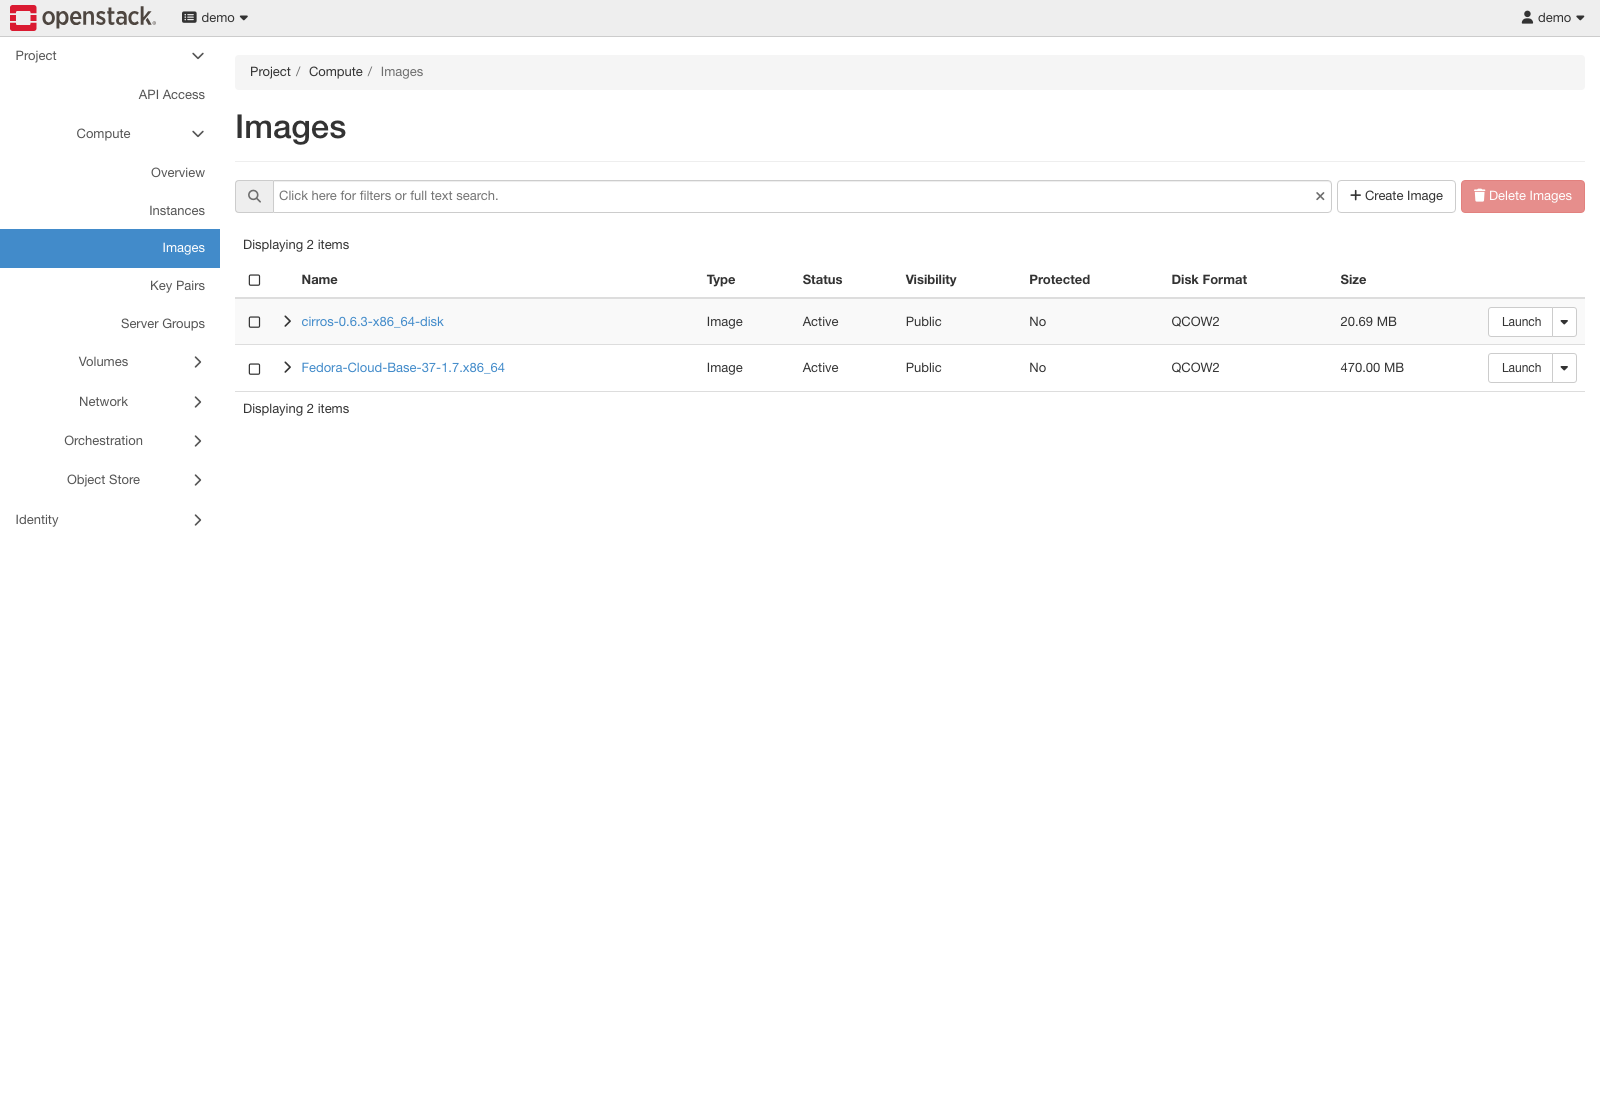
\includegraphics[width=0.88\linewidth]{img/m1-glance-image-catalog.png}
\caption{Kho lưu trữ ảnh hệ điều hành Glance đã nạp CirrOS và Fedora.}
\label{fig:m1_glance_images}
\end{figure}

\begin{itemize}
    \item \textbf{Hạ tầng Mạng ảo \& Subnet (Hình~\ref{fig:m1_networks} và~\ref{fig:m1_subnets}):} Neutron đã khởi tạo sẵn các phân đoạn mạng cơ sở gồm các mạng nội bộ tenant (\texttt{private}, \texttt{shared}, \texttt{heat-net}) và mạng ngoại vi (\texttt{public}). Phân đoạn \texttt{private-subnet} được cấu hình dual-stack hỗ trợ cả IPv4 (\nolinkurl{10.0.0.0/26}) và IPv6 (\nolinkurl{fd52:aee0:36f2::/64}).
\end{itemize}

\begin{figure}[H]
\centering
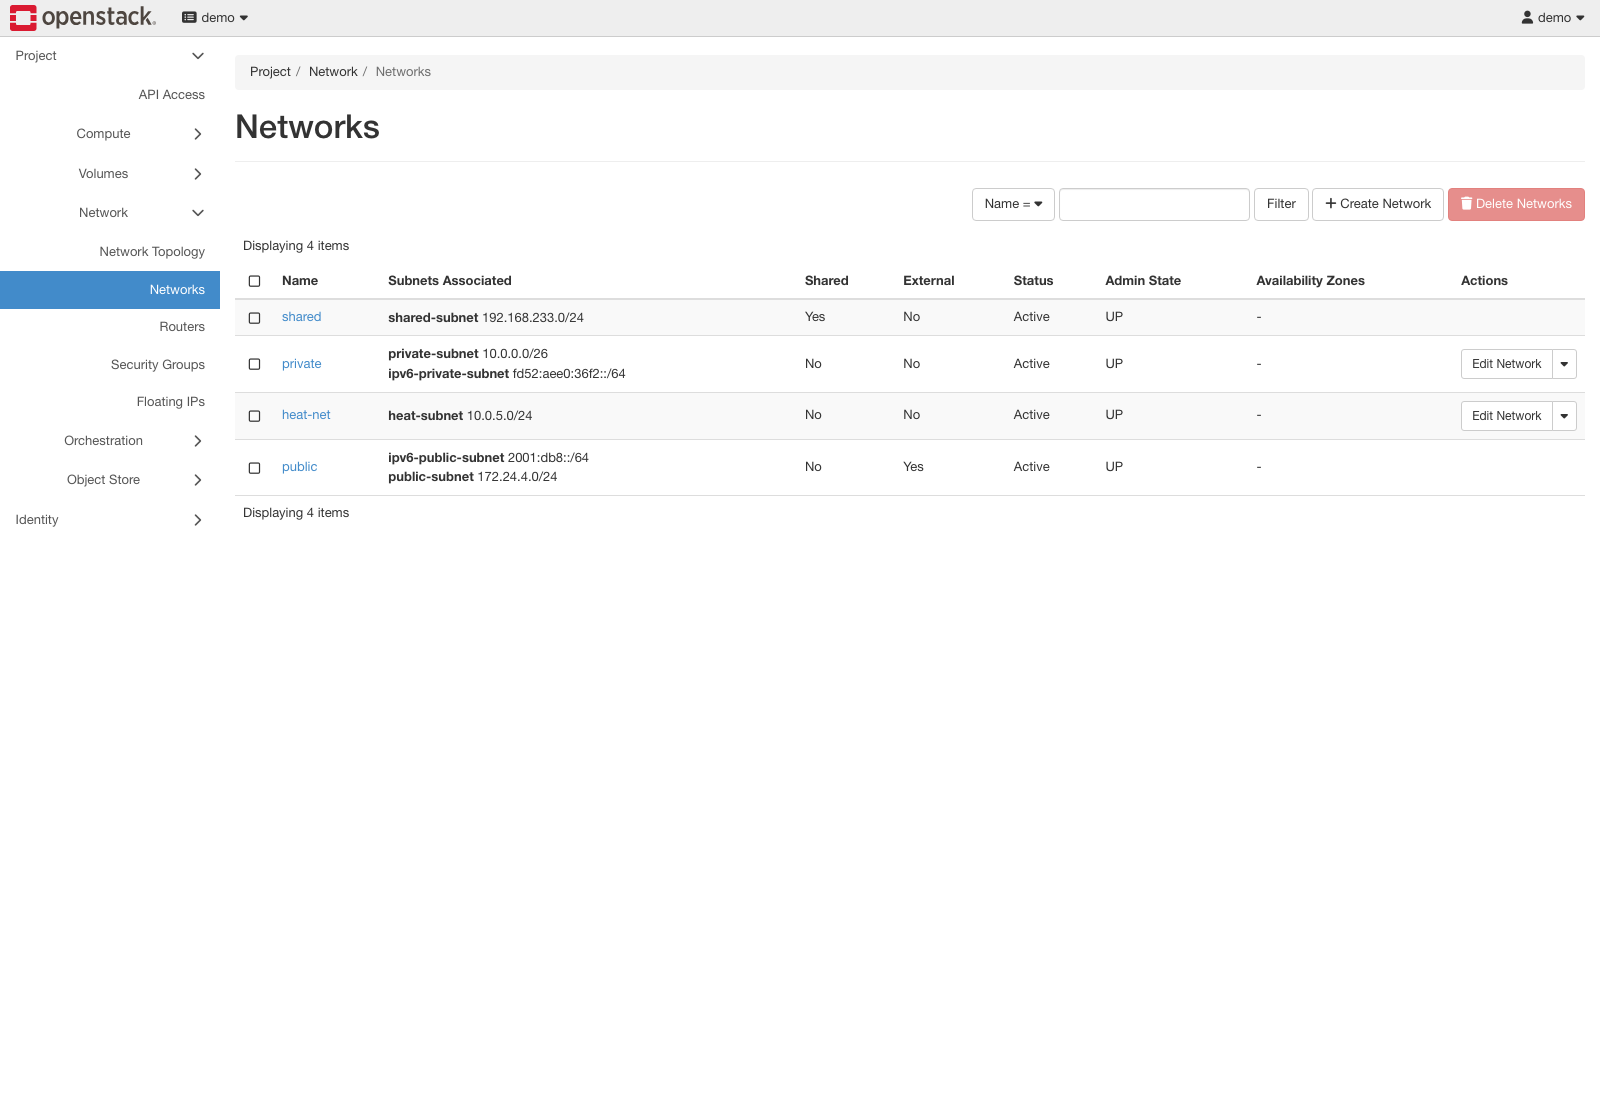
\includegraphics[width=0.88\linewidth]{img/m1-neutron-networks-list.png}
\caption{Danh sách mạng ảo hóa trong Neutron chi tiết các phân đoạn mạng.}
\label{fig:m1_networks}
\end{figure}

\begin{figure}[H]
\centering
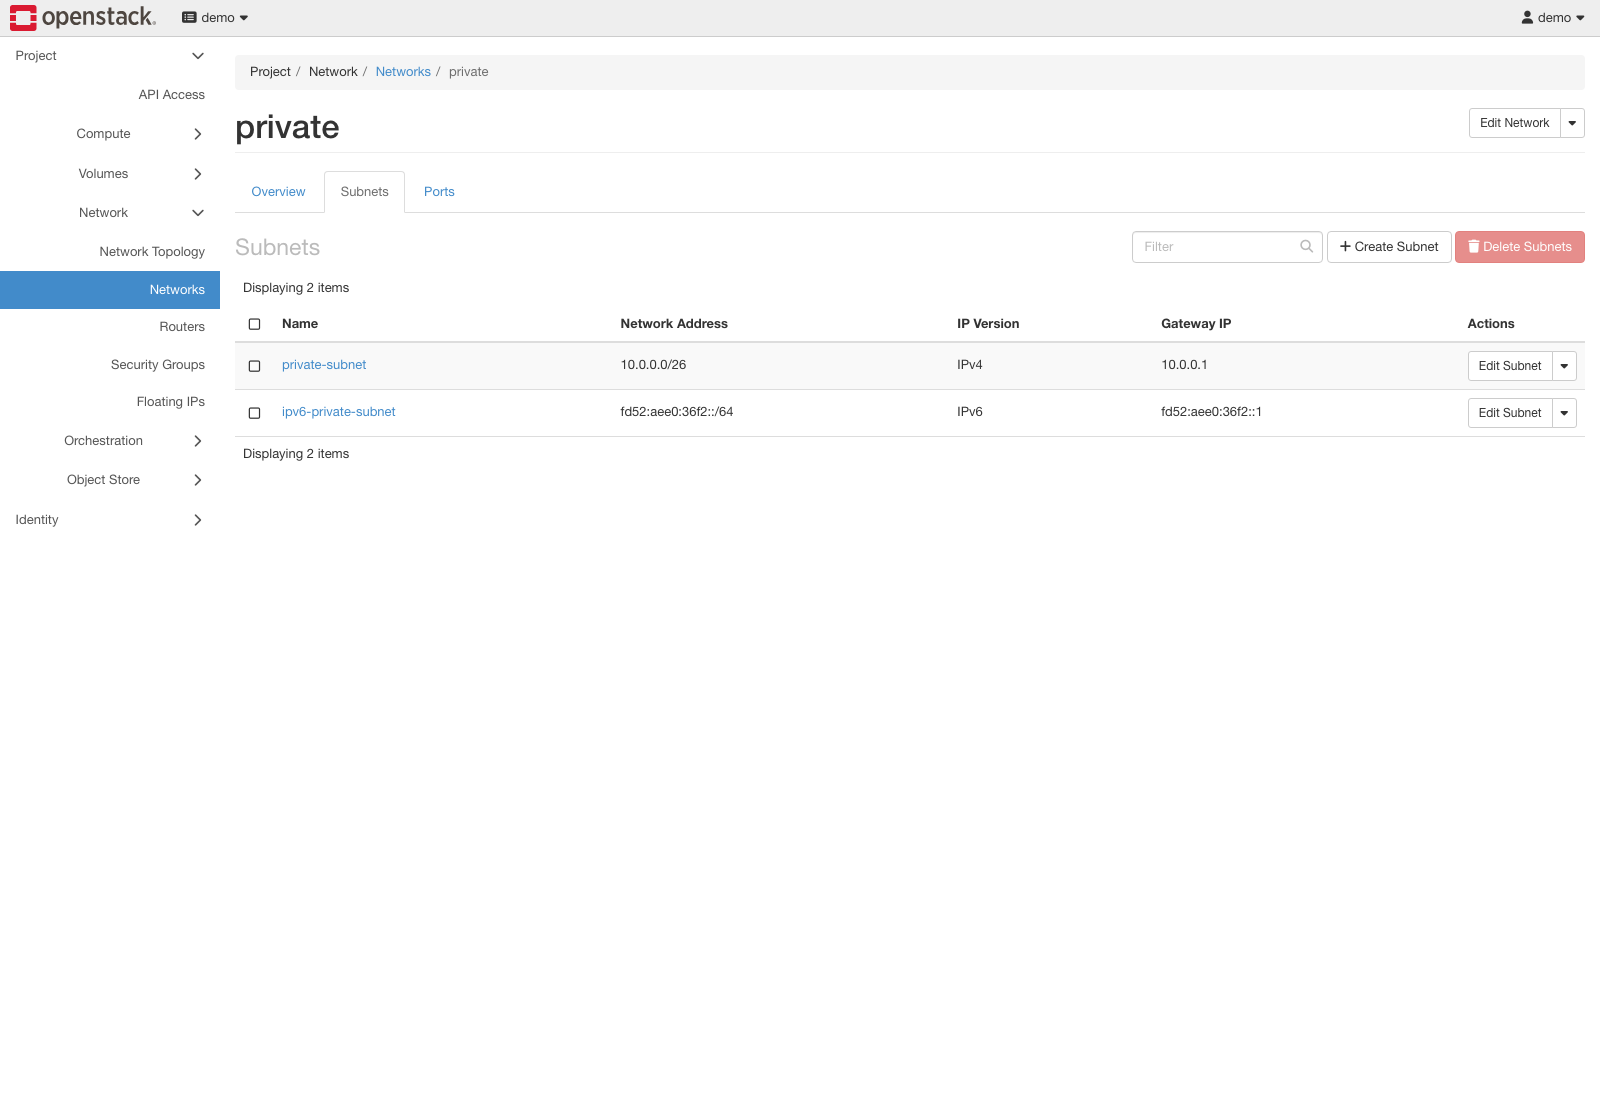
\includegraphics[width=0.88\linewidth]{img/m1-neutron-subnets-detail.png}
\caption{Chi tiết cấu hình dải địa chỉ Subnet trên mạng \texttt{private}.}
\label{fig:m1_subnets}
\end{figure}

\begin{itemize}
    \item \textbf{Bộ định tuyến L3 ảo (Hình~\ref{fig:m1_routers}):} Bộ định tuyến mặc định \texttt{router1} đang hoạt động ở trạng thái \texttt{Active}, được gắn sẵn cổng Gateway hướng ra mạng ngoài \texttt{public}.
    \item \textbf{Nhóm Bảo mật (Hình~\ref{fig:m1_secgroups}):} Nhóm tiến hành rà soát các luật tường lửa mặc định trong nhóm \texttt{default} để nắm rõ chính sách lưu lượng trước khi triển khai thêm các quy tắc mới.
\end{itemize}

\begin{figure}[H]
\centering
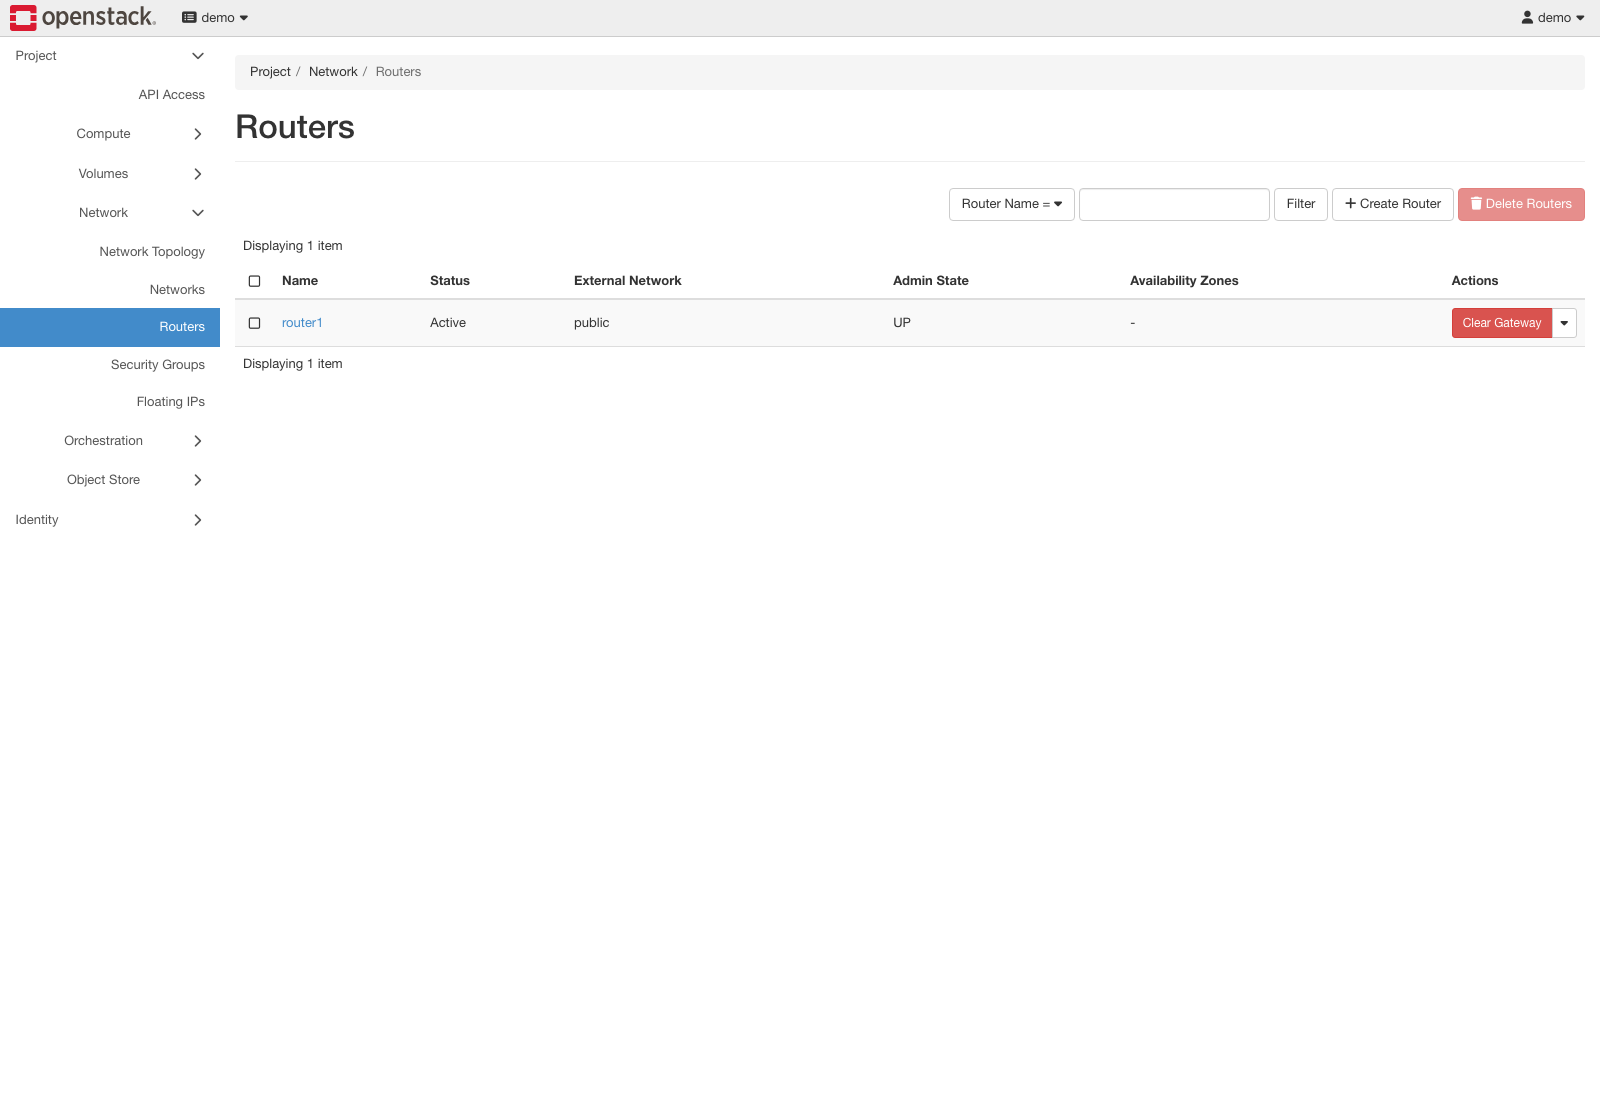
\includegraphics[width=0.88\linewidth]{img/m1-neutron-router-overview.png}
\caption{Bộ định tuyến \texttt{router1} kết nối Gateway ngoại vi ra mạng \texttt{public}.}
\label{fig:m1_routers}
\end{figure}

\begin{figure}[H]
\centering
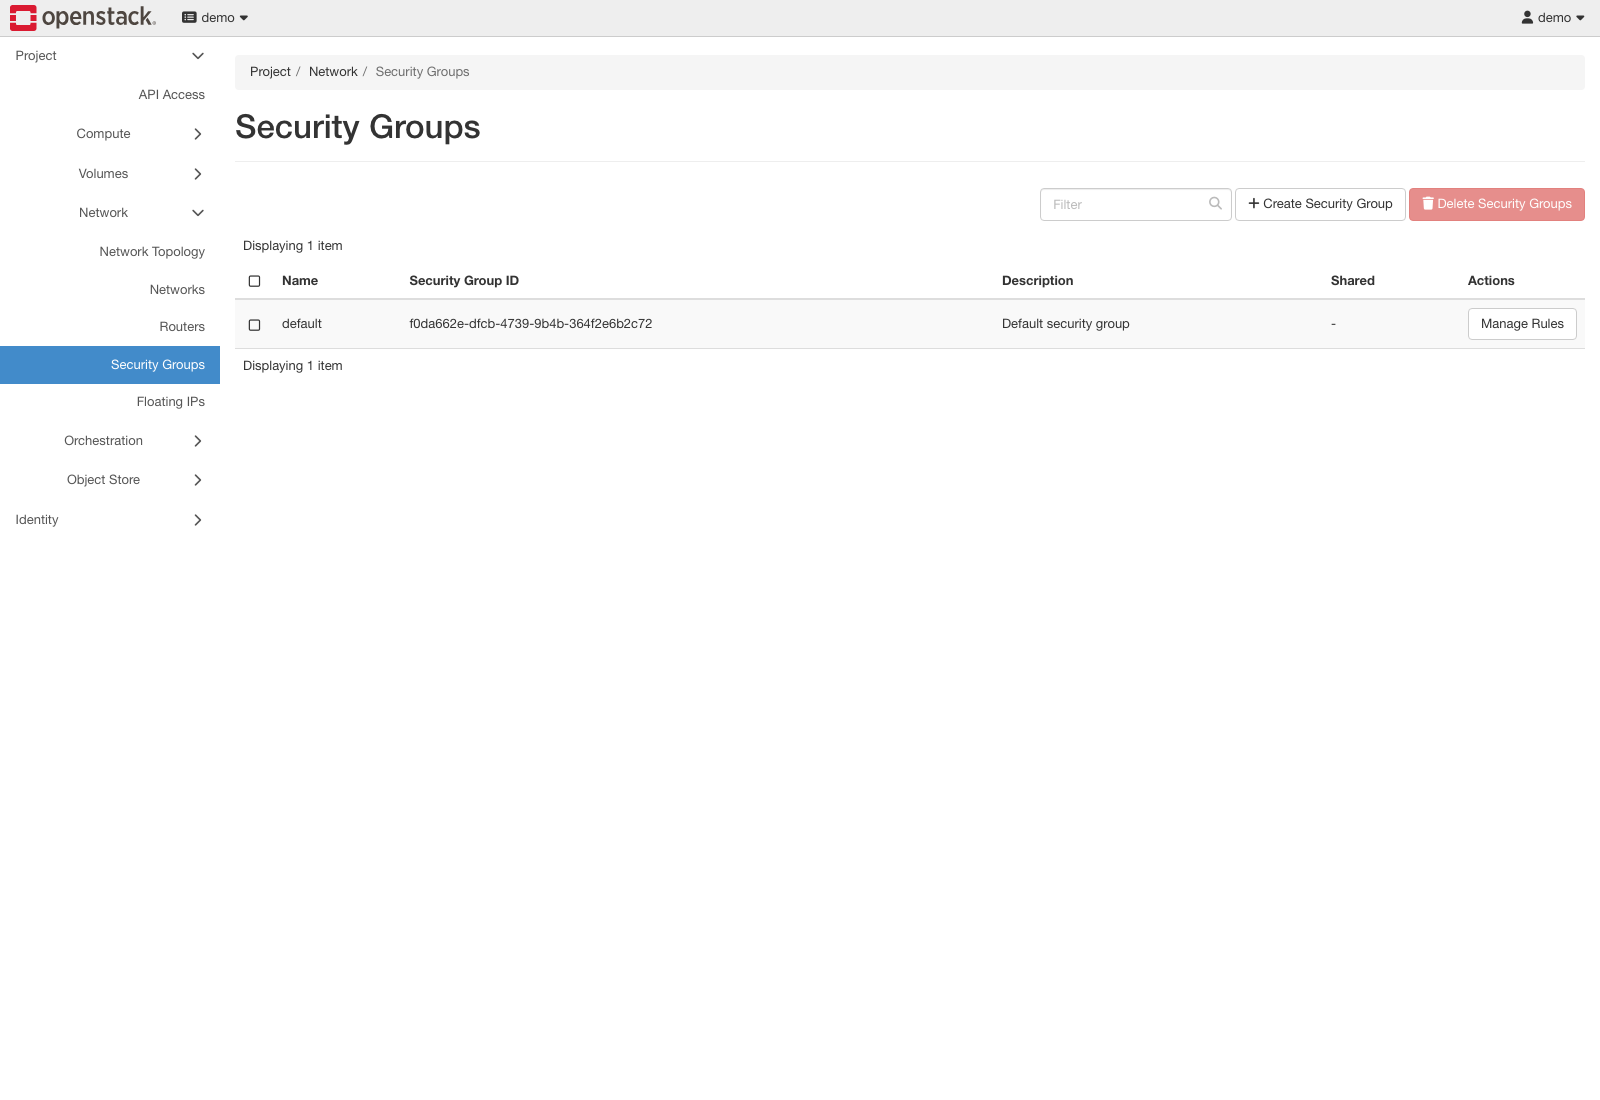
\includegraphics[width=0.88\linewidth]{img/m1-neutron-security-groups.png}
\caption{Bảng luật tường lửa Security Groups mặc định của dự án.}
\label{fig:m1_secgroups}
\end{figure}

\begin{itemize}
    \item \textbf{Khóa SSH \& Heat Stacks (Hình~\ref{fig:m1_keypairs} và~\ref{fig:m1_heat_stacks}):} Khảo sát danh mục SSH Keypair cũng như trạng thái ban đầu của bảng quản lý Heat Orchestration Stacks trước khi nạp template.
    \item \textbf{Lưu trữ Đối tượng Swift (Hình~\ref{fig:m1_swift_containers}):} Xác nhận dịch vụ Swift Object Storage đã sẵn sàng tiếp nhận yêu cầu tạo container và lưu trữ dữ liệu.
\end{itemize}

\begin{figure}[H]
\centering
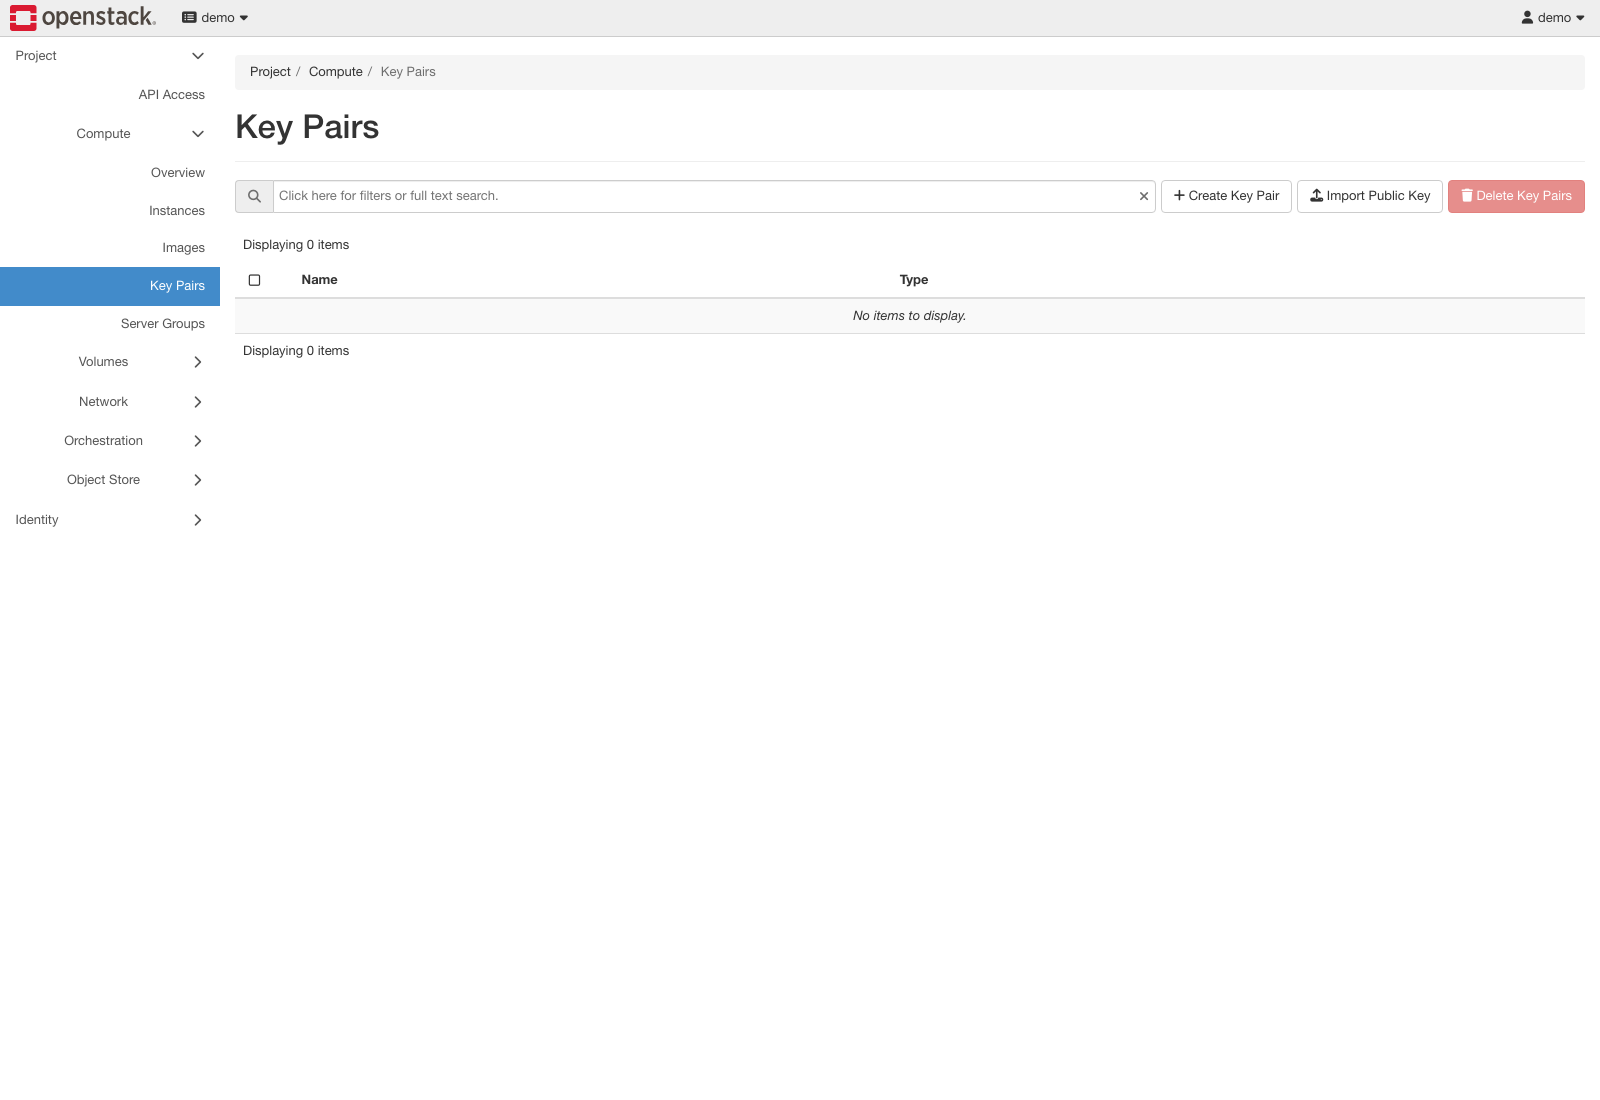
\includegraphics[width=0.88\linewidth]{img/m1-nova-keypairs-list.png}
\caption{Giao diện quản lý SSH Key Pairs trong Nova Compute.}
\label{fig:m1_keypairs}
\end{figure}

\begin{figure}[H]
\centering
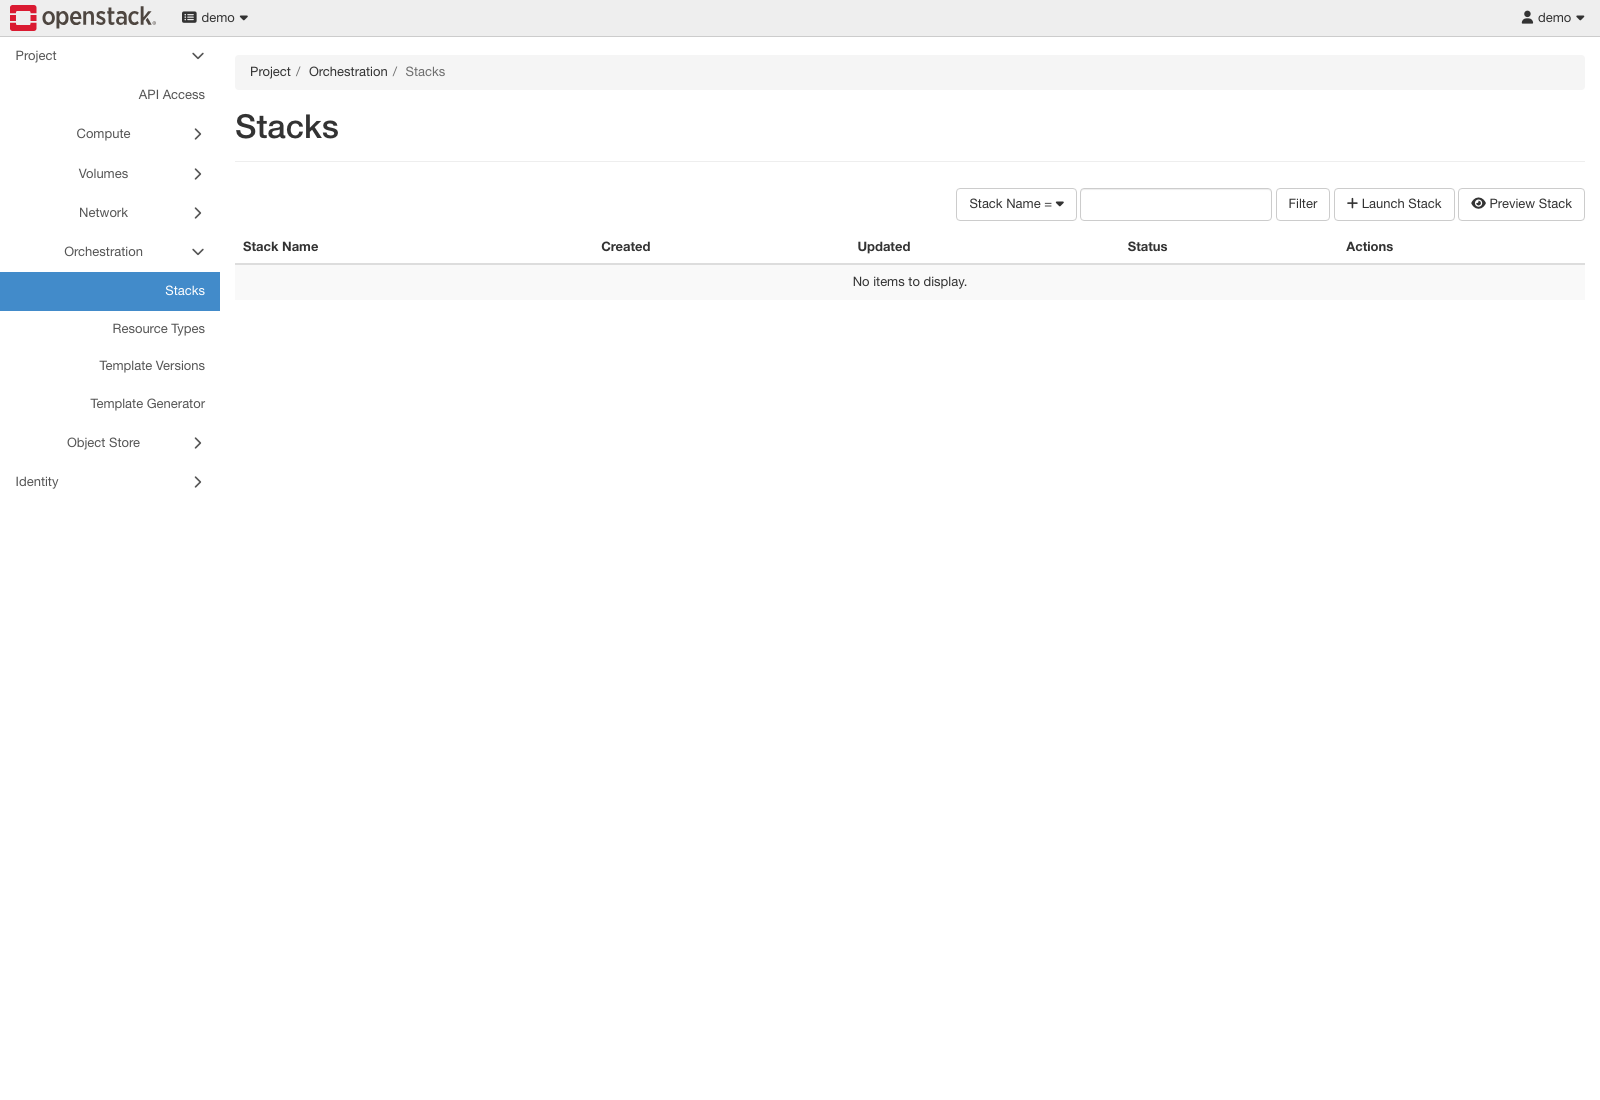
\includegraphics[width=0.88\linewidth]{img/m1-heat-stacks-initial.png}
\caption{Bảng điều khiển Heat Orchestration Stacks ở trạng thái ban đầu.}
\label{fig:m1_heat_stacks}
\end{figure}

\begin{figure}[H]
\centering
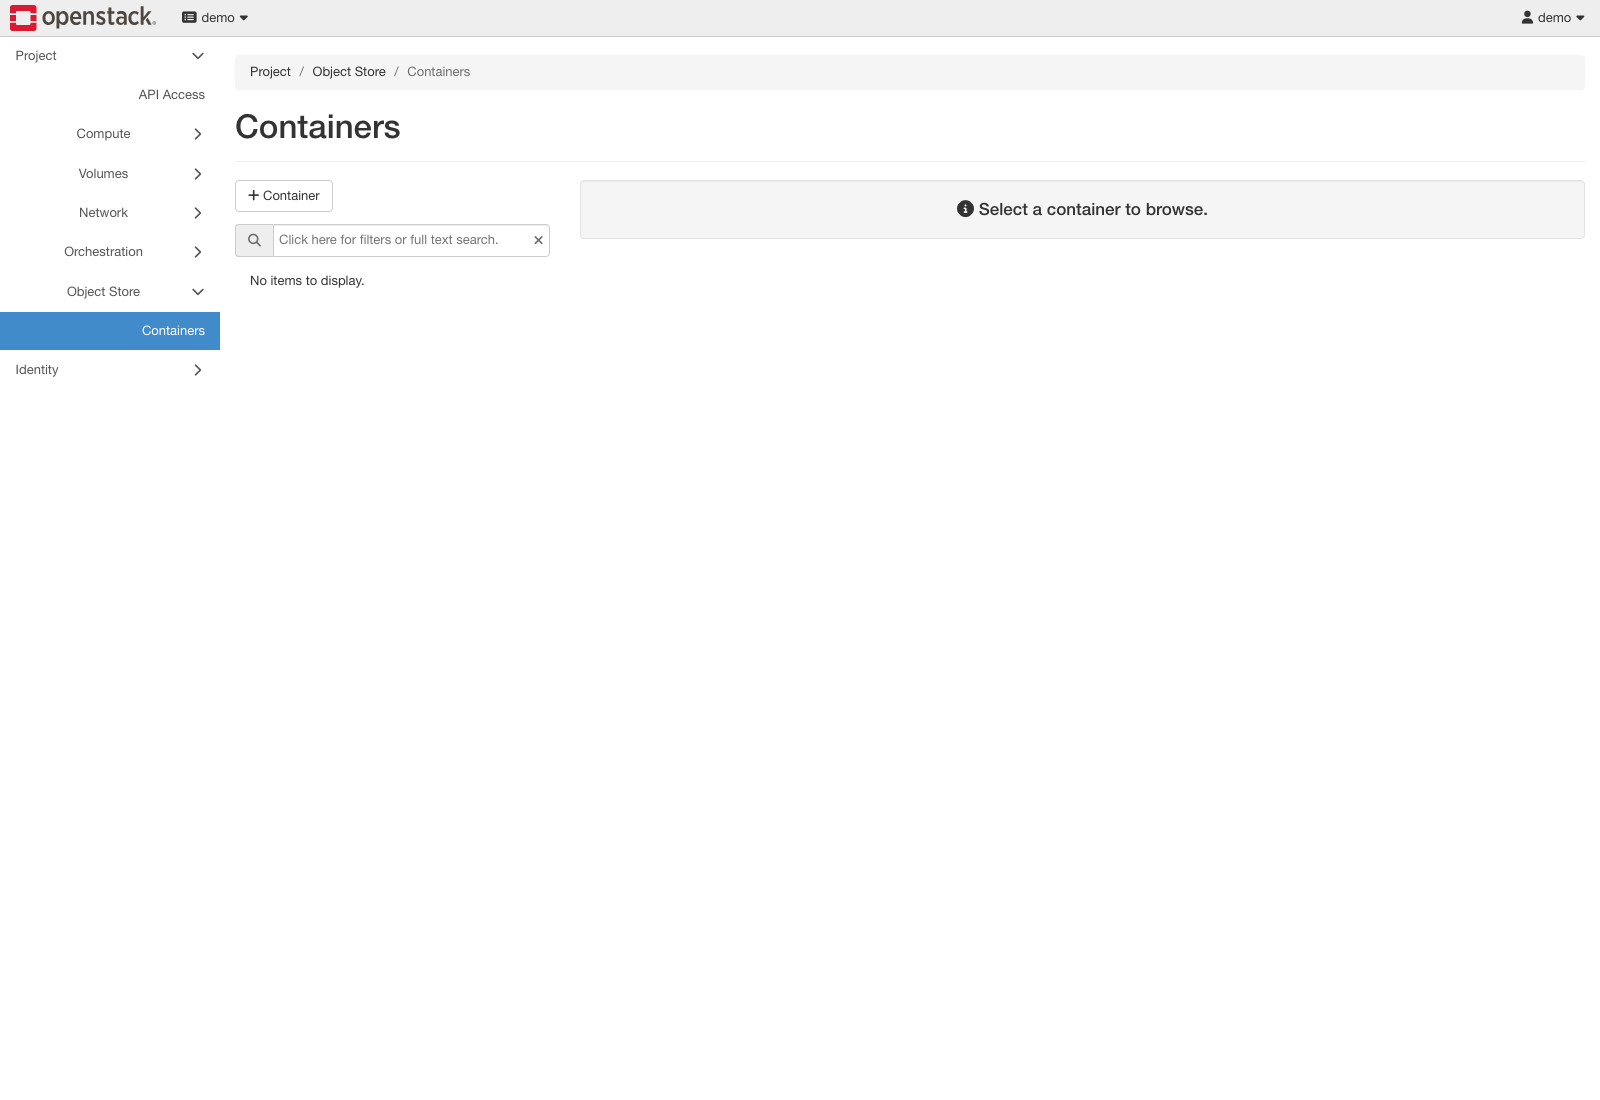
\includegraphics[width=0.88\linewidth]{img/m1-swift-containers-initial.png}
\caption{Bảng điều khiển Swift Object Storage trước khi khởi tạo vùng lưu trữ.}
\label{fig:m1_swift_containers}
\end{figure}

\subsection{Vòng đời Máy ảo: Khởi tạo, Kiểm tra Runtime \& Hủy Cấp phát}
Để kiểm chứng trọn vẹn vòng đời máy ảo cũng như quy trình lập lịch của Nova, nhóm chúng em tiến hành khởi tạo một máy ảo thử nghiệm mang tên \nolinkurl{module1-horizon-instance} thông qua wizard trên giao diện Horizon (Hình~\ref{fig:m1_launch_dialog}):
\begin{itemize}
    \item \textbf{Cấu hình khởi tạo:} Nhóm lựa chọn gói tài nguyên tối thiểu Flavor \texttt{m1.nano} (1 vCPU, 64 MB RAM, 1 GB Disk), sử dụng ảnh nguồn \nolinkurl{cirros-0.6.3-x86_64-disk} và kết nối vào mạng nội bộ \texttt{private}.
    \item \textbf{Kiểm tra trạng thái runtime (Hình~\ref{fig:m1_instance_active}):} Quá trình cấp phát diễn ra thuận lợi; máy ảo nhanh chóng chuyển sang trạng thái \texttt{Active} với Power State là \texttt{Running}, được gán địa chỉ IP nội bộ \texttt{10.0.0.45} (IPv4) và \nolinkurl{fd52:aee0:36f2:0:f816:3eff:fed0:3caa} (IPv6).
    \item \textbf{Hủy cấp phát và thu hồi tài nguyên (Hình~\ref{fig:m1_delete_confirmation} và~\ref{fig:m1_instances_empty}):} Sau khi kiểm tra xong, nhóm thực hiện thao tác xóa máy ảo. Giao diện Horizon cập nhật danh sách máy ảo về trạng thái rỗng, qua đó xác nhận hệ thống đã giải phóng hoàn toàn các tài nguyên vCPU, RAM và cổng mạng ảo về lại quota chung của dự án.
\end{itemize}

\begin{figure}[H]
\centering
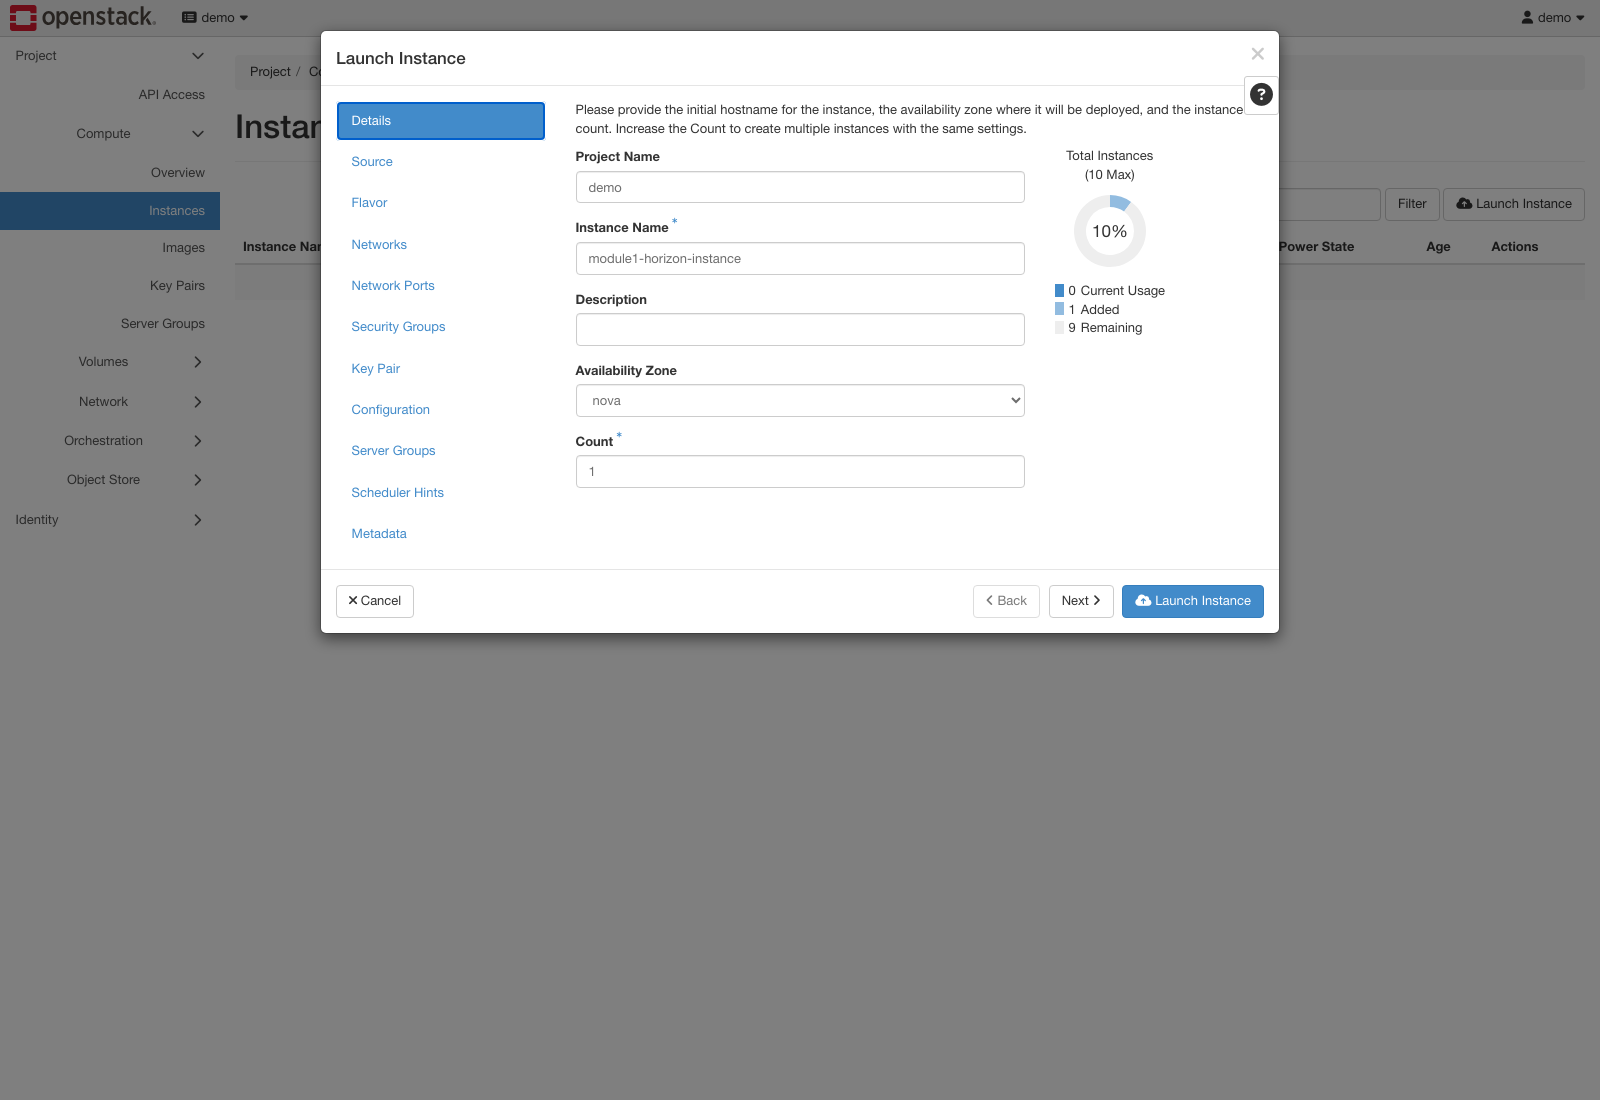
\includegraphics[width=0.88\linewidth]{img/m1-instance-launch-wizard.png}
\caption{Wizard khởi tạo máy ảo trong Horizon thể hiện các thông số cấu hình.}
\label{fig:m1_launch_dialog}
\end{figure}

\begin{figure}[H]
\centering
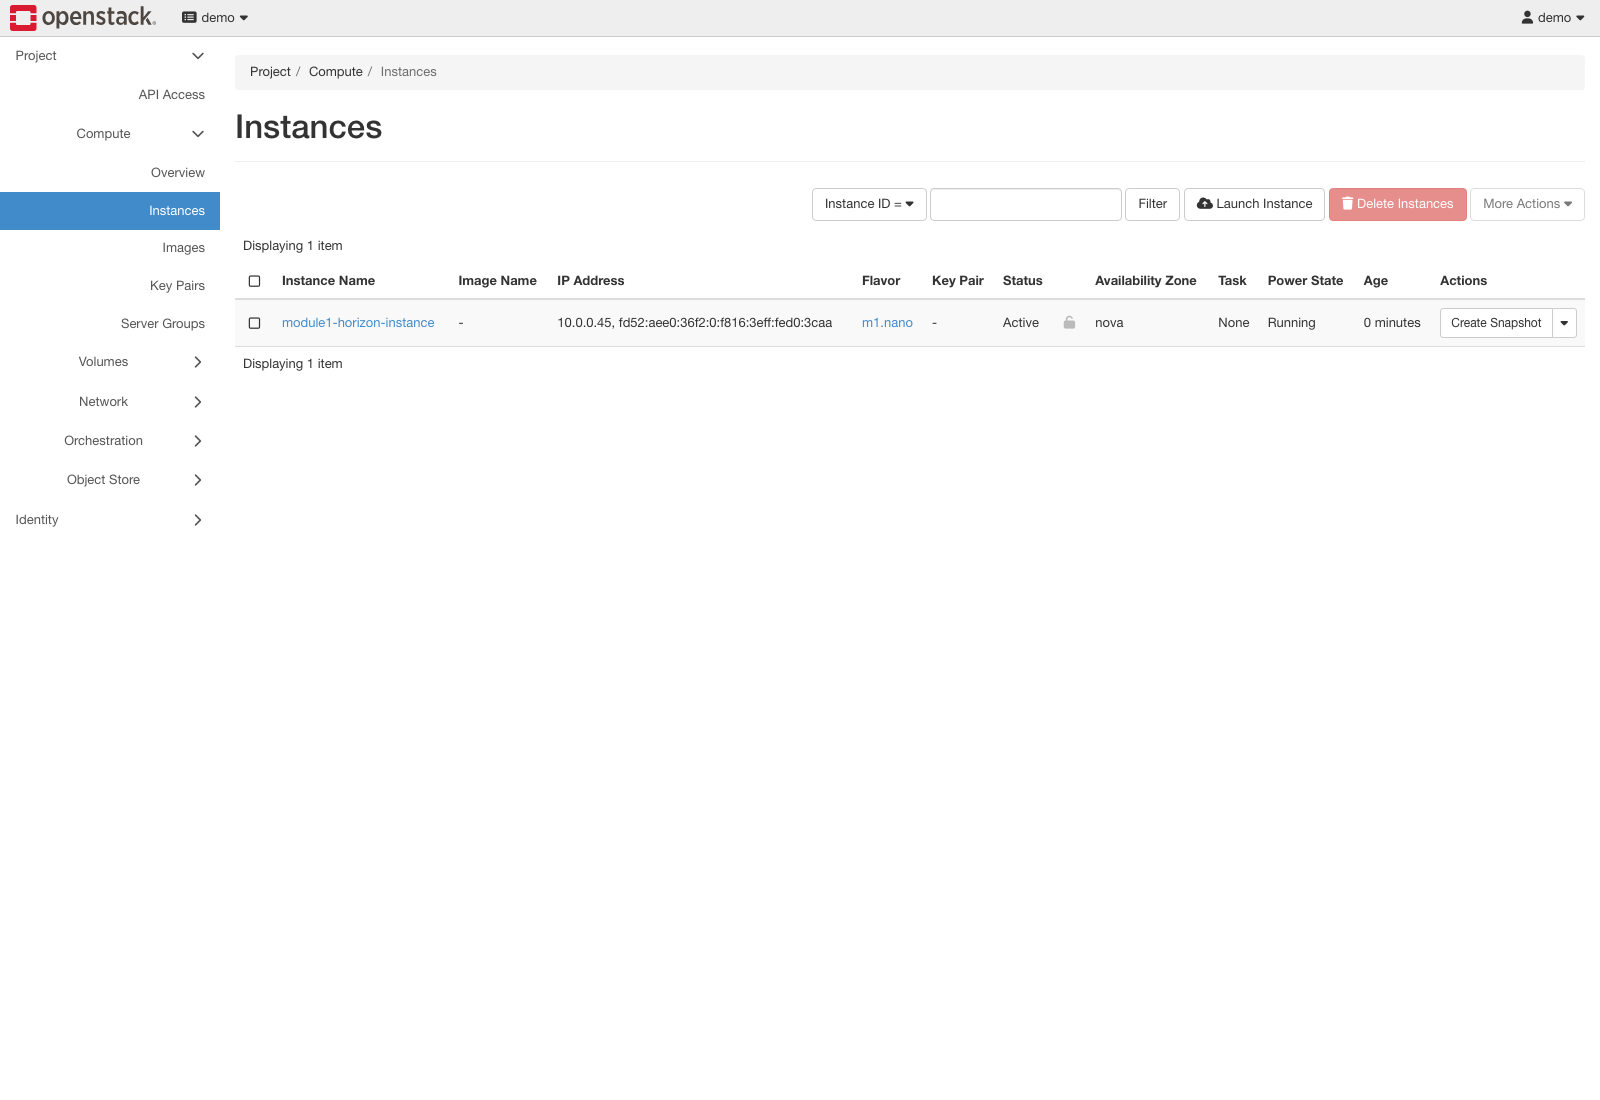
\includegraphics[width=0.88\linewidth]{img/m1-instance-active-status.png}
\caption{Máy ảo đạt trạng thái Active với Power State Running trong Nova.}
\label{fig:m1_instance_active}
\end{figure}

\begin{figure}[H]
\centering
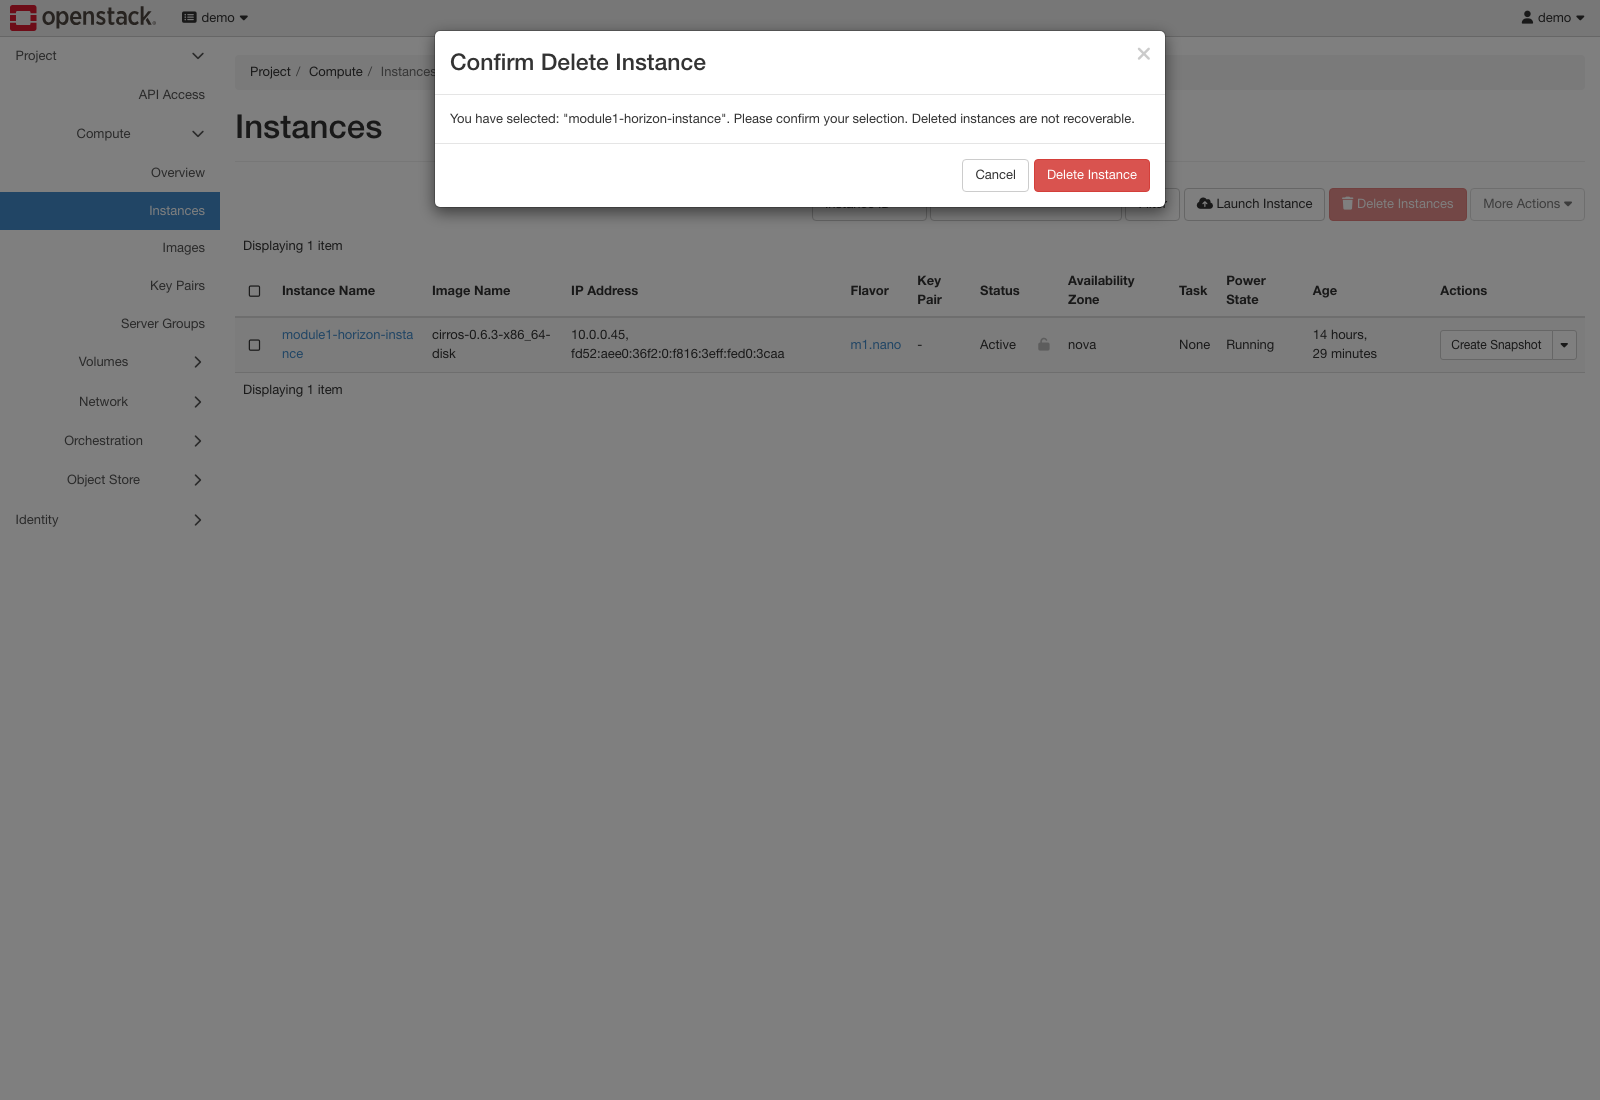
\includegraphics[width=0.88\linewidth]{img/m1-instance-delete-confirmation.png}
\caption{Modal xác nhận xóa máy ảo \nolinkurl{module1-horizon-instance}.}
\label{fig:m1_delete_confirmation}
\end{figure}

\begin{figure}[H]
\centering
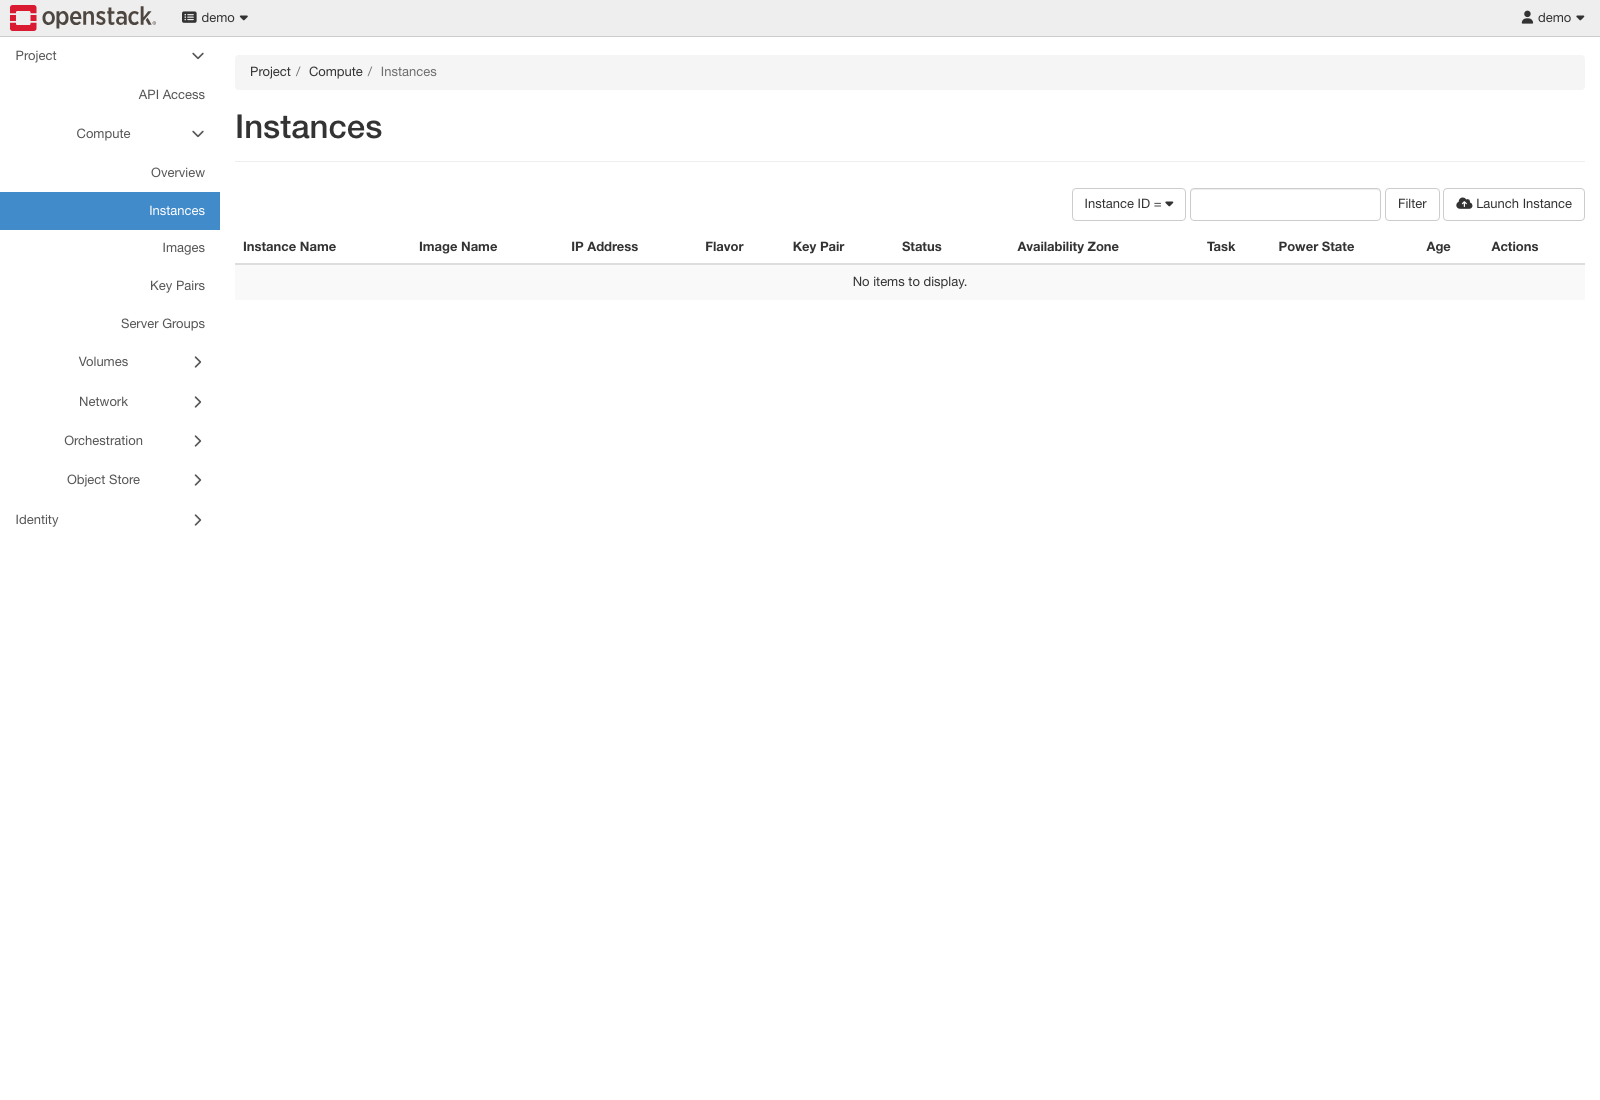
\includegraphics[width=0.88\linewidth]{img/m1-instance-terminated-empty.png}
\caption{Danh sách máy ảo rỗng sau khi thu hồi tài nguyên thành công.}
\label{fig:m1_instances_empty}
\end{figure}
